%% Elsevier 'elsarticle' template — Structures (review mode)
\pdfminorversion=7 % allow inclusion of up to PDF 1.7 graphics
\documentclass[review,12pt]{elsarticle} % ilk gönderimde review + tek sütun
\journal{Structures}
\biboptions{square}

%% Packages
\usepackage[english]{babel}
\usepackage{amsmath,amssymb,mathtools}
\usepackage{graphicx}
\usepackage{siunitx}
\usepackage{microtype}
\makeatletter
\AtBeginDocument{\@ifundefined{MT@orig@showhyphens}{}{\let\showhyphens\MT@orig@showhyphens}}
\makeatother
\usepackage{lineno}
\usepackage{booktabs}
\usepackage{tabularx}
\usepackage{array}
\usepackage{ragged2e} % daha iyi satır sonu için (opsiyonel)
\usepackage{placeins}



%% siunitx
\sisetup{
mode = match,
propagate-math-font = true,
reset-math-version = false,
reset-text-family = false,
reset-text-series = false,
reset-text-shape = false,
text-family-to-math = true,
text-series-to-math = true,
per-mode = symbol,
range-units = single,
range-phrase = --,
exponent-product = \times
}

%% Microtype
\microtypesetup{expansion,protrusion}
\emergencystretch=3em
\allowdisplaybreaks[1]

% --- HYPERREF EN SONDA ---
\usepackage{hyperref}
\makeatletter
\pdfstringdefDisableCommands{%% disable front-matter commands in PDF strings
\def\corref#1{}
\def\cortext#1{}
\def\cnotenum#1{}
\def\@corref#1{}
}
\makeatother
\newcolumntype{L}{>{\RaggedRight\arraybackslash}X}
\providecommand*{\theHpage}{\thepage}

\begin{document}
\pagenumbering{roman}
\renewcommand*{\theHpage}{FR\roman{page}}
\begin{frontmatter}

\title{Hydro--thermal high-fidelity modelling and multi-objective design of fluid viscous dampers}

%% Authors
\author[aff1]{Ad Soyad\corref{cor1}}
\ead{email@kurum.edu.tr}
\cortext[cor1]{Corresponding author.}

\address[aff1]{Bölüm, Kurum, Şehir, Posta Kodu, Türkiye}

%% Abstract
\begin{abstract}
% 150–250 kelime: Amaç; hidrolik–termal FVD modeli (Cd(Re), kavitasyon, μ(T));
% 10-DOF yapısal model ve zaman entegrasyonu; çok-amaçlı GA (⟨IDR⟩, ⟨PFA⟩);
% başlıca bulgular (yüzdesel azaltımlar, güvenlik metrikleri); pratik tasarım ilkeleri.
\end{abstract}

%% Graphical abstract (ayrı PDF/PNG ekleyebilirsin)
\begin{graphicalabstract}
% \includegraphics[width=\linewidth]{figs/graphical_abstract.pdf}
\end{graphicalabstract}

%% Highlights (3–5 madde)
\begin{highlights}
\item Physics-informed fluid viscous damper with Cd(Re), cavitation soft-limit and two-node thermal coupling.
\item 10-DOF shear-frame under PSA-band scaled ground motions; robust time integration.
\item NSGA-II based multi-objective design reduces both IDR and PFA while satisfying hydraulic/thermal safety.
\end{highlights}

%% Keywords
\begin{keyword}
Fluid viscous damper \sep seismic optimization \sep Cd(Re) \sep cavitation \sep thermal coupling \sep NSGA-II
\end{keyword}
\end{frontmatter}

\hypersetup{pageanchor=false}
\clearpage
\pagenumbering{arabic}
\renewcommand*{\theHpage}{MA\arabic{page}}
\hypersetup{pageanchor=true}


%% ---------------- Main text ----------------
\section{Introduction}
Earthquake engineering has progressively shifted from strength-based checks to performance-based design, yet modern buildings in high seismic regions still struggle to control interstorey drifts and peak floor accelerations under rare but intense ground motions. Even when global strength and code-level ductility demands are satisfied, excessive interstorey drift ratios (IDR) can trigger damage in non-structural components and architectural finishes, while large peak floor accelerations (PFA) amplify the vulnerability of suspended ceilings, façades, contents and sensitive equipment, leading to disproportionate economic and functional losses. To mitigate these demands without resorting to prohibitively stiff or massively over-strengthened lateral systems, a broad family of supplemental damping devices has been developed, including metallic yielding dampers, friction devices, tuned mass dampers and base-isolation systems, alongside velocity-dependent fluid viscous dampers (FVDs) that are now widely deployed in buildings and bridges as robust passive energy dissipation elements \cite{Zoccolini2023,Frings2017,Zhang2024}. In current practice, design codes such as EN~15129 and ASCE~7 explicitly recognise FVDs and largely treat them through equivalent viscous damping and simple power-law force–velocity relations of the form $F = C \lvert v \rvert^{\alpha}$, with constant $(C,\alpha)$ pairs calibrated from qualification tests and then used in equivalent SDOF or low-order MDOF models for time-history analysis \cite{sist:2018:en15129,asce7,Cetin2019,AhadzadehKolour2021}. This article acknowledges the practical success of such phenomenological representations and their role in reducing IDR and PFA in many realised projects, but argues that the internal hydro–thermal behaviour of FVDs (pressure limits, flow capacity, cavitation and temperature-driven viscosity loss) and its interaction with multi-record, multi-objective design at building level have so far been treated only in a fragmented way, without a unified framework that links device-scale physics to system-scale performance and safety metrics.

Most analytical and design-oriented studies still represent fluid viscous dampers with a phenomenological power–law dashpot of the form
$F_\mathrm{vd} = C\,|\dot u|^{\alpha}\operatorname{sgn}(\dot u)$, sometimes combined with simple floor-wise placement rules for linear or nonlinear devices.\citep{Kolour2021,Cetin2019,Deringol2021,Arjmand2024,Zoccolini2023}
This class of models is attractive because it introduces only a few parameters, can be identified directly from full-scale hysteresis loops, and can be embedded in nonlinear response-history analysis without additional internal state variables.
Full-scale component tests typically report almost rectangular force–displacement cycles and mechanically stable $(C,\alpha)$ pairs over a wide range of amplitudes and frequencies,\citep{Tang2021} which reinforces the impression that a single effective power law is sufficient for engineering design.
At the same time, detailed CFD and rheology-based studies show that this apparent simplicity masks a strong sensitivity to internal flow mechanisms: for nominally similar devices, changes in orifice layout, flare angle and shear-thinning behaviour can move the effective velocity exponent anywhere between about $0.2$ and $1.0$, and substantially alter the force–velocity backbone.\citep{Agha2023}
In other words, the laminar gap flow and jet-orifice losses are lumped into one “black-box” dashpot, and neither pressure nor temperature appears explicitly in the state description.

A second modelling line replaces the pure dashpot by a Maxwell-type combination of a nonlinear dashpot and an axial spring, or by an equivalent complex stiffness in the frequency domain.
Such models reproduce frequency-dependent stiffness and the “inflated” force–velocity loops observed in large-scale tests much more accurately than a memoryless dashpot and, when coupled with adaptive time-integration schemes, they keep numerical errors at the level of only a few percent even for very stiff, strongly nonlinear devices.\citep{Akcelyan2018,Dong2022}
Nevertheless, the damper is still treated as a single-input–single-output element whose behaviour is calibrated solely against global $F$–$u$ or $F$–$\dot u$ loops; internal pressure, flow capacity or local cavitation are not resolved.
A third group of models introduces explicit hysteresis through Bouc–Wen-type or related differential laws, including specialised formulations proposed for fluid viscous dampers that can match pinching, strength degradation and production scatter across multiple specimens within a single parameter set.\citep{Cucuzza2023,DeDomenico2019,Kolour2021}
These advanced phenomenological models offer a richer and statistically more robust description of device-level energy dissipation, yet they still operate at the level of an effective restoring force and do not provide direct access to hydro–thermal quantities that are critical for device integrity.

Across all three families, some physically important aspects therefore remain systematically outside the design loop.
Typical formulations do not enforce explicit limits on internal pressure at seals or cylinders, do not track the ratio between instantaneous flow and a realistic capacity $Q/Q_\mathrm{cap}$, and do not include cavitation onset or temperature-driven viscosity loss as hard constraints in the optimisation of damper parameters or layouts.
Instead, such checks—when performed at all—are usually deferred to separate qualification tests on a small number of prototypes.
This leaves a gap between current phenomenological, Maxwell and hysteretic representations and a truly physics-based description in which pressure, flow saturation, cavitation and thermal thinning enter the state vector and the objective functions of the design problem, a gap that motivates the hydro–thermal modelling framework developed in this study.

A smaller but rapidly growing body of work has tried to open the ``black box'' of fluid viscous dampers and resolve the underlying thermo–hydraulic processes that are hidden behind simple $F=C|\dot u|^{\alpha}$ laws.
Early theoretical studies by Black and Makris showed that, under highly idealised long–duration pulses, internal oil temperatures could in principle rise well above $200\,^\circ\mathrm{C}$, with a corresponding loss of damping capacity \citep{BlackMakris2007}.
More recent full–scale experiments have largely corrected this picture for building–type demands: Laka and Zahrai report that typical earthquake–like histories only heat a commercial device by about $2$–$3\,^\circ\mathrm{C}$, whereas $O(10^3)$–cycle harmonic protocols can drive the temperature increase up to $\sim 50\,^\circ\mathrm{C}$ and noticeably weaken the force–velocity response \citep{Lak2023}.
Complementary gap–type damper tests and thermo–mechanical models indicate that, under more extreme but still experimentally accessible loading, internal pressures may reach the order of $10^2$~MPa, local oil temperatures can approach or exceed $200\,^\circ\mathrm{C}$, and the dynamic viscosity may drop by roughly one order of magnitude; in those regimes, measured peak forces have been observed to degrade by about $20\%$ over a single long test \citep{Zhang2024}.
On the modelling side, high–fidelity CFD and thermo–hydraulic studies have resolved laminar and jet branches, Reynolds–dependent discharge coefficients and heat transfer within the damper, often using Carreau–Yasuda rheology and compressible fluid laws \citep{Frings2017,Agha2023}.
These works convincingly demonstrate that the effective $(C,\alpha)$ pair is highly sensitive to geometry, rheology and temperature, and that ignoring thermo–mechanical coupling can bias the inferred supplemental damping ratio by about $10$–$12\%$ in multi–degree–of–freedom analyses \citep{Hu2025}.
However, almost all of these studies remain at specimen scale, or at most consider a single prototype structure under a handful of sinusoidal or recorded excitations.
When FVDs are embedded in building or bridge models, the devices are usually collapsed back to isothermal phenomenological elements and only structural metrics such as inter–storey drift, peak floor acceleration or damage indices are tracked \citep{AhadzadehKolour2021,Cetin2019,Bakhshinezhad2020,Arjmand2024}.
To the best of the authors' knowledge, there is still no framework that simultaneously (i) retains a physics–based hydro–thermal damper model with explicit pressure, flow and temperature histories, (ii) couples this model to a realistic multi–storey frame subjected to an intensity–measure–controlled set of real ground motions, and (iii) embeds hydraulic and thermal safety indicators—such as pressure capacity, flow throttling, cavitation onset or viscosity fade—directly into a multi–objective design problem alongside conventional response measures.

To organise these ingredients into a single workflow, the present study adopts a three-phase hydro–thermal, safety-driven design framework, sketched in Figure~\ref{fig:overall_workflow}, which progresses from input preparation and ground-motion processing (Phase~1) through GA setup and definition of decision variables, objectives and safety constraints (Phase~2) to the optimisation loop and Pareto-front extraction (Phase~3).

\begin{figure}[h!]
  \centering
  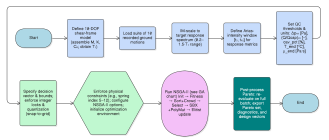
\includegraphics[width=\linewidth]{Genel.pdf}
  \caption{Overall methodological workflow: (Phase 1) input preparation and ground-motion processing, (Phase 2) GA setup and definition of decision variables, objectives and safety constraints, and (Phase 3) optimisation loop and Pareto-front extraction.}
  \label{fig:overall_workflow}
\end{figure}
\FloatBarrier

Against this backdrop, the present paper proposes a hydro--thermal, safety–driven design framework for FVD‐equipped shear buildings that explicitly links device‐scale physics with multi–record, performance–based seismic assessment. First, we formulate a reduced–order fluid viscous damper model that separates laminar gap and orifice jet branches, assigns a Reynolds–dependent discharge coefficient with a soft–min cavitation limiter, and couples a two–node thermal block to temperature–dependent viscosity and density, so that pressure, flow and temperature histories are tracked consistently while the damper is embedded in the equations of motion of a 10‐DOF shear frame; in contrast to earlier CFD and thermo–hydraulic studies conducted at specimen level \citep{Agha2023,Lak2023,Frings2017}, the proposed model is deliberately kept ODE‐based and inexpensive enough for large sets of ground motions. Second, we adopt a band–averaged geometric mean spectral acceleration centred at the first–mode period as intensity measure, and we evaluate all response and device metrics within a common Arias window $[t_5,t_{95}]$ (including peak floor accelerations, interstorey drifts, pressure percentiles, $Q/Q_{\mathrm{cap}}$, cavitation ratio, end–of–record temperature and viscosity), thereby extending Sa,avg–type IMs and significant–duration concepts \citep{Vargas-Alzate2022,Davatgari-Tafreshi2023} to a joint assessment of structural performance and internal damper safety. Third, we cast the FVD design problem as a lexicographic, multi–objective optimisation in a 12–dimensional space of orifice geometry, piston/spring parameters and thermal properties, where an aggregated penalty $f_{\mathrm{pen}}$ that counts hydraulic and thermal QC violations is minimised first and only then average peak floor accelerations and interstorey drifts are traded off via NSGA–II; this safety–first formulation goes beyond existing multi–objective or risk–informed designs that tune simple power–law or Maxwell–type dampers at structural level without enforcing explicit pressure, cavitation or temperature limits \citep{Kolour2021,Bakhshinezhad2020,Zhong2020,Arjmand2024}. Finally, we interrogate the resulting Pareto fronts to extract engineering patterns---in particular, that near–optimal solutions tend to cluster around medium piston diameters, multiple small orifices, intermediate oil viscosity and moderate heat–transfer capacity—and we discuss how such patterns can be distilled into design charts or surrogate models that complement current code–oriented practice and placement studies \citep{Cetin2019,SiamiKaleybar2021,Farahpour2023}; although the present work is restricted to a planar shear archetype with a single damper configuration, the framework is purposely formulated so that it can be extended to three–dimensional buildings with torsion, multiple damper layouts, semi–active valve laws and life–cycle or ageing costs in the objective set.

% --- BIBLIOGRAPHY SECTION (REVISED) ---
\bibliographystyle{elsarticle-num}

\IfFileExists{bibtext2.bib}{%
  \bibliography{bibtext2}%
}{%
  % If 'bibtex.bib' is not found, it prints a placeholder
  \begin{thebibliography}{00}
  \bibitem[{Placeholder(2025)}]{placeholder2025}
  Placeholder Author, ``CRITICAL ERROR: 'bibtext2.bib' file not found. Please create it and add BibTeX entries,'' (2025).
  \end{thebibliography}%
}

\end{document}
